\section{Solução para Automação do Processo de Medição da Qualidade Interna do Produto}
\label{sec:solucao}

Visando atingir a automação do processo de medição de qualidade interna do produto por meio de técnicas não intrusivas no ambiente de desenvolvimento de software, realizou-se uma revisão bibliográfica da literatura em busca de ambientes de informação permitissem o uso de ferramentas (não-intrusivas) para automatizar a coleta e o uso de sofisticadas técnicas de análise de dados \cite{Gopal2005} . Trabalhos como o de Palza \cite{Palza2003},  Ruiz \cite{Ruiz2005}, Castellanos \cite{Castellanos2005},  Becker \cite{Becker2006}, Folleco \cite{Folleco2007} e Silveira \cite{Silveira2010}, evidenciaram que ambientes de \textit{Data Warehousing} são boas soluções para se automatizar um programa de métricas em processos de desenvolvimento de software.

\textit{Data Warehousing} é uma coleção de tecnologias de suporte à decisão disposta a capacitar os responsáveis por tomar decisões a fazê-las de forma mais rápida \cite{chaudhuri1997} \cite{andre2000}. Em outras palavras, trata-se de um processo para montar e gerenciar dados vindos de várias fontes, com o objetivo de prover uma visão analítica de parte ou do todo do negócio em repositório central chamado de \textit{data warehouse} \cite{gardner1998} \cite{Kimball2002}. A arquitetura de um ambiente de \textit{data warehousing} pode ser vista na Figura \ref{arquitetura}. 

\begin{figure}[ht!]
\centering
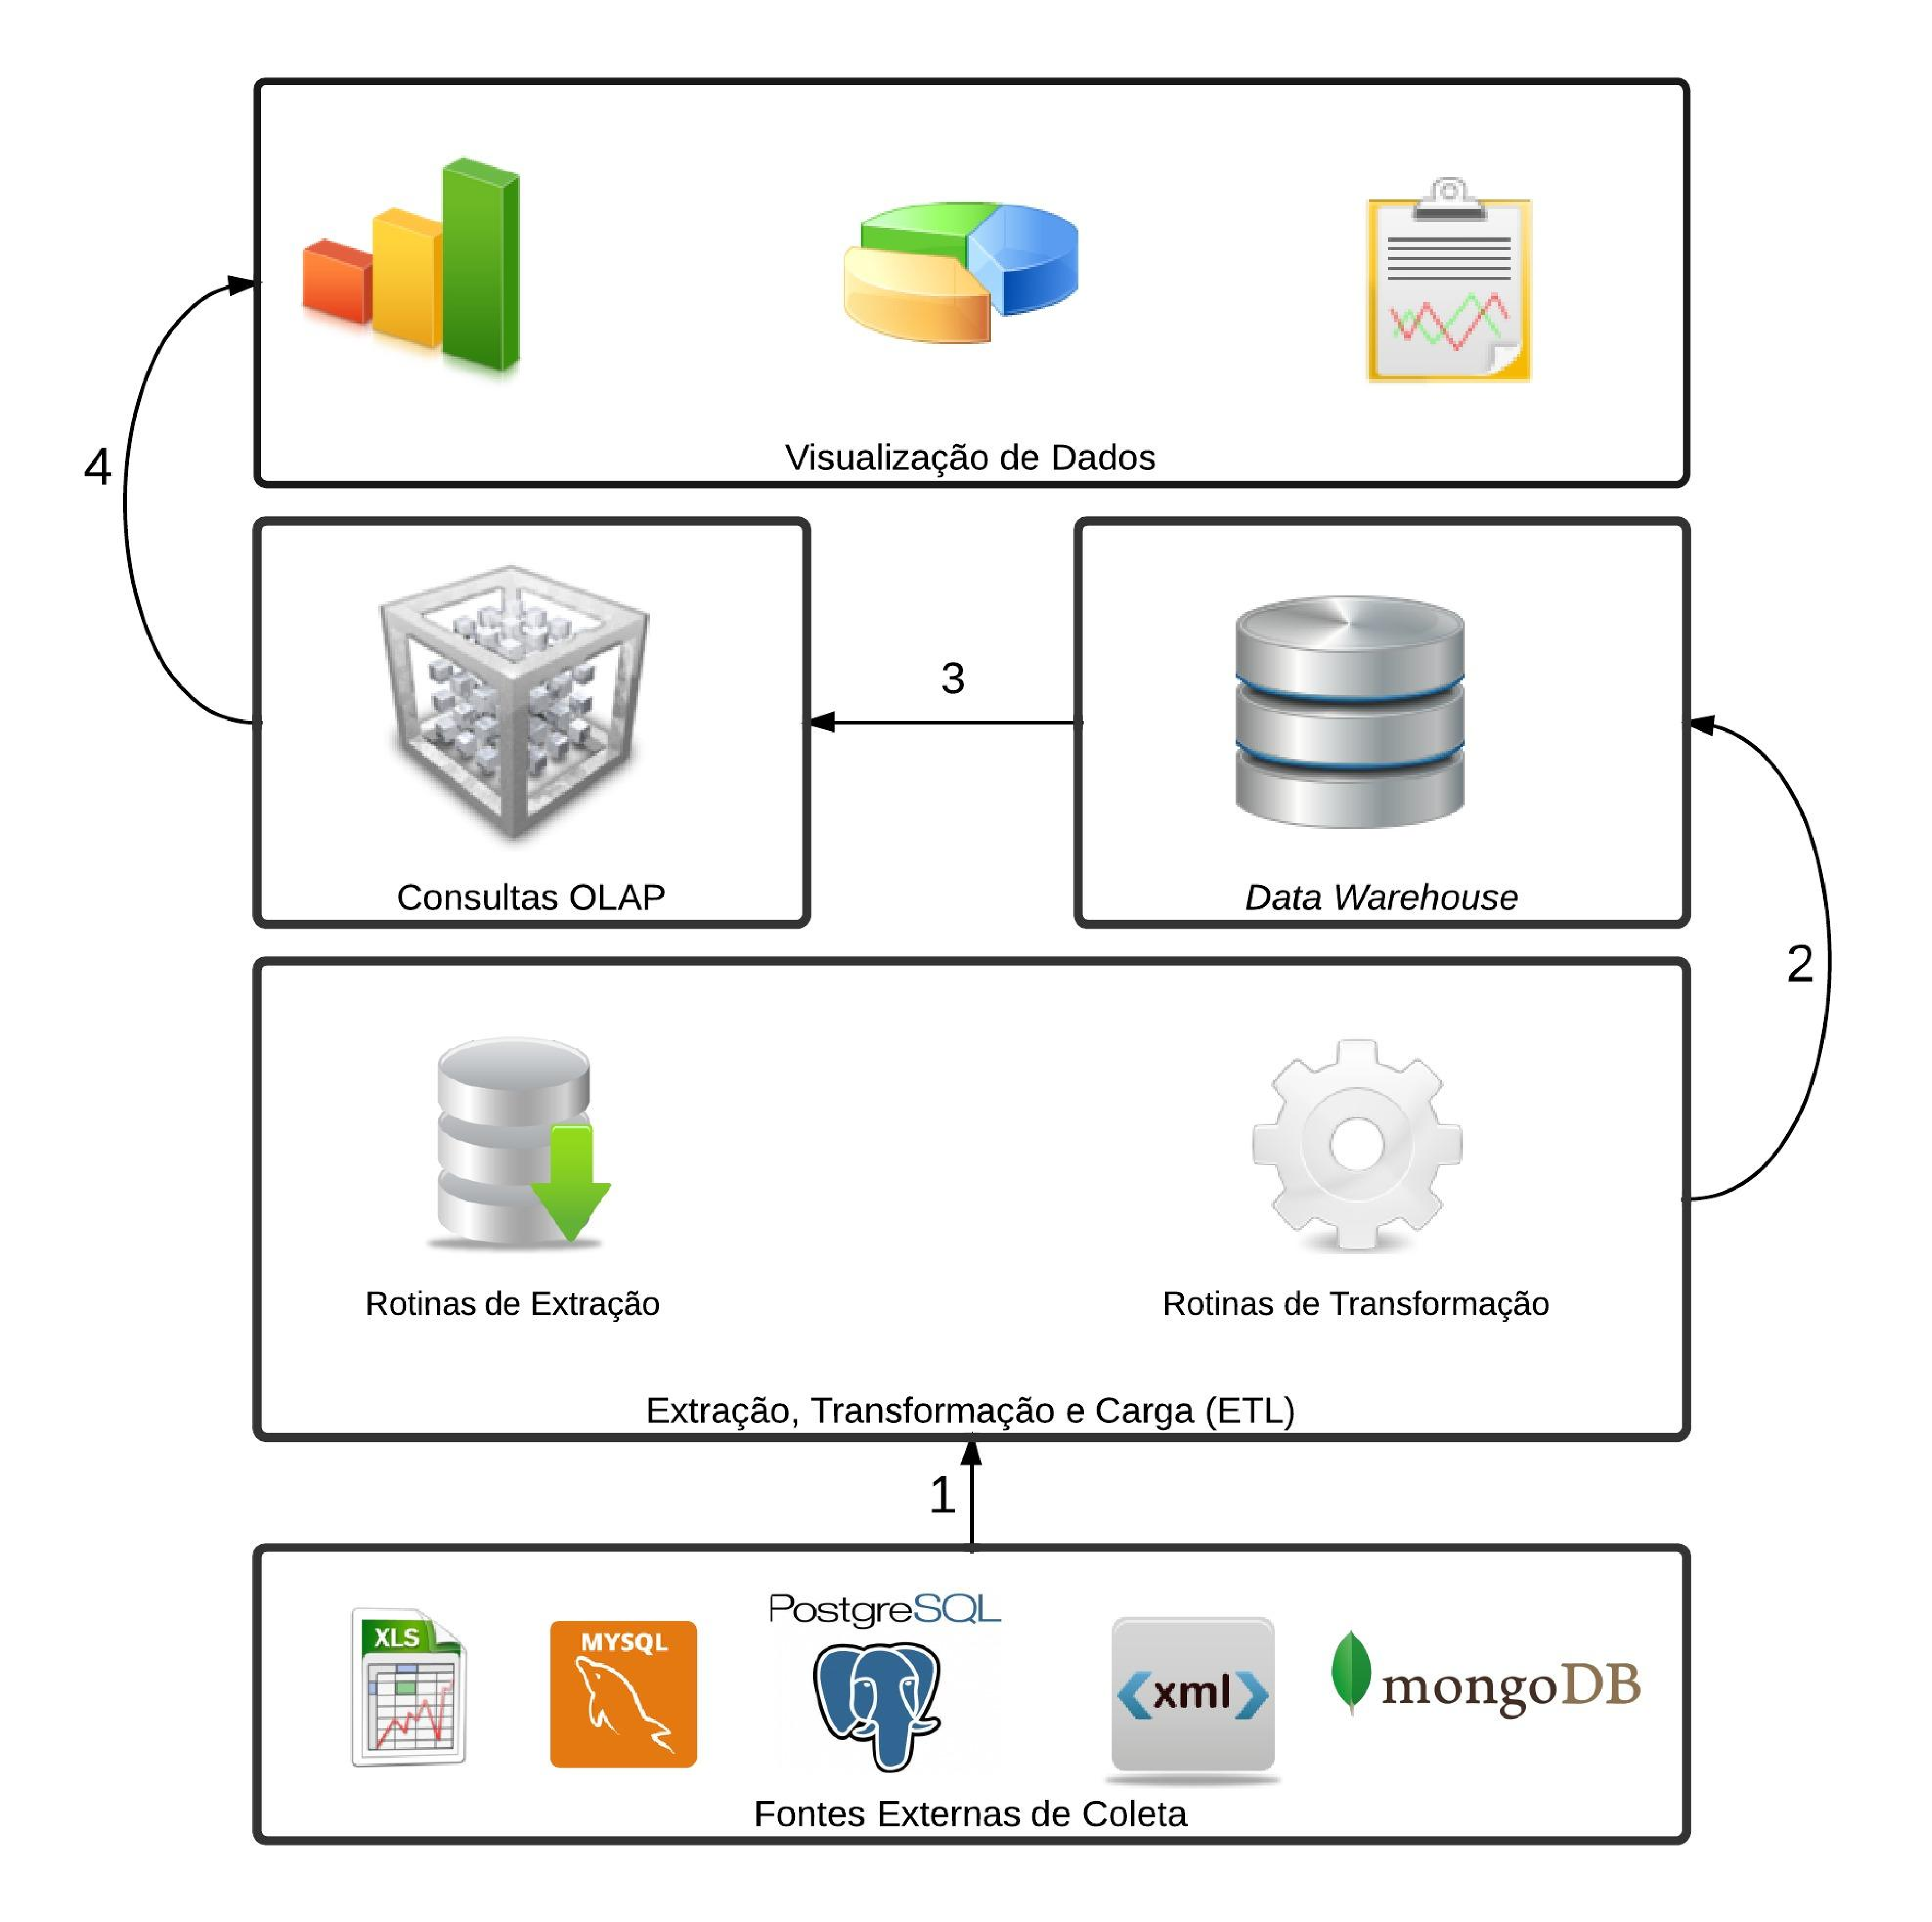
\includegraphics[keepaspectratio=false,scale=0.14]{figuras/Dwing.eps}
\caption{Arquitetura do Ambiente de \textit{Data Warehousing}}
\label{arquitetura}
\end{figure}
\FloatBarrier


Na Figura \ref{arquitetura}, as setas 1 e 2 representam o processo de \textit{Extraction-Transformation-Load (ETL)} que é o processo de extração, transformação e carga dos dados de forma automática e não instrusiva ao ambiente de desenvolvimento. Este processo pode consumir até 85\% de todo o esforço em um ambiente de \textit{Data Warehousing} \cite{Kimball2002}; A seta 3 representa as consultas \textit{On-Line Analytical Processing (OLAP)} que são operações de consulta e análise flexíveis realizadas sobre \textit{data warehouse}projetado sobre um modelo dimensional \cite{Kimball2002} \cite{Codd1993}; A seta 4 representa a visualização dos dados em forma de gráficos, tabelas ou painéis customizáveis conhecidos como \textit{dashboards}.


A implementação do ambiente de \textit{data warehousing} mostrado na figura \ref{arquitetura} se deu pela ferramenta Analizo\footnote{Disponível em \url{http:/http://analizo.org/}}, responsável por coletar as métricas de código-fonte, a suite Pentaho BI Community\footnote{Disponível em \url{http://community.pentaho.com/}}, que dispõe de ferramentas de ETL e OLAP, um banco de dados MariaDB\footnote{Disponível em \url{http://mariadb.org/}} modelado sobre um modelo dimensional e o plugin Saiku Analitics\footnote{Disponível em \url{http://meteorite.bi/saiku}} para visualização de dados. 